\chapter{Proposed implementation}
\label{chap:impl}

My goal is to design and implement library for \acrlong{acc:ea}, as mentioned in the chapter \ref{chap:eva}. The library should not only implement existing \acrshortpl{acc:ea} and allow to execute them on the \gpuns, but also afford general framework to which it would be simple to plug new algorithms. For the user of the library should be easy to replace evolutionary operators, modify them or if necessary replace the whole workflow of the algorithm.

I decide to implement the library using Pipe and Filter architecture as specified by \citet{EnterpriseIntegrationPatterns}. The example of this architecture is in figure \ref{fig:pipesandfilters}. The general idea is to partition the algorithm into smaller, simple steps and use the output of one step as the input to the following one. \acrshort{acc:ea} are simple to split, as one step may be one evolutionary operator. I decided to implement the library in the \enquote{Convention over Configuration} design pattern -- that is the operators make same assumptions about the format and order of the input, rather than explicitly specifying it in the configuration. I still provide ways to control the parameters, if required by the user, and I will get to it a bit later.

\begin{figure}
    \centering
    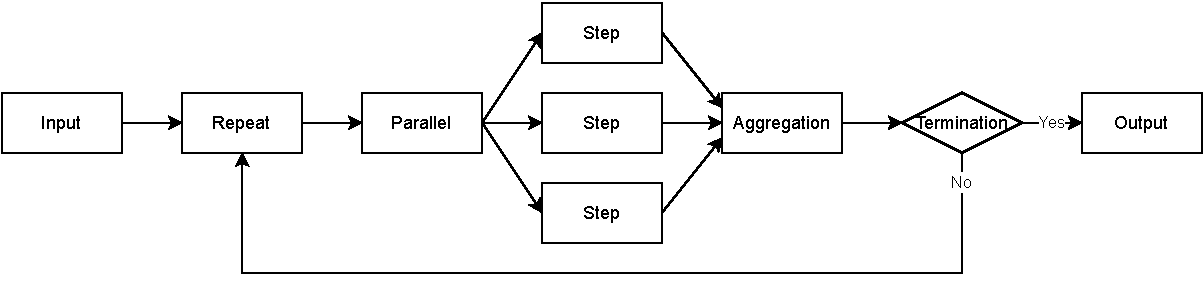
\includegraphics[width=\textwidth]{img/PipesAndFilters.pdf}
    \caption{Pipe and Filter architecture}
    \label{fig:pipesandfilters}
\end{figure}

The pure Pipe and Filter architecture is not sufficient for implementation of \acrshort{acc:ea}. In the purest implementation, this architecture is just chain of steps following each other. I decide to expand it by a number of useful steps like loops, parallel step invocation and more. Example of parallel step respectively loop use in the Pipe and Filter architecture is demonstrated in figure \ref{fig:pipesandfilters}. The parallel invocation is designed in the figure by \enquote{Parallel} block, followed by the \enquote{Aggregation} block accumulating the results from each step. The loop is represented by the \enquote{Repeat} block accompanied by the \enquote{Termination} block controlling the termination condition of the loop.

My proposed implementation is the \emph{\acrfull{acc:ffeat}}. This library is attached to this work, available on my GitHub account \citep{FFEATrepo}, and ready for install as PyPI (Python Package Index) \href{https://pypi.org/project/FFEAT/}{package}. The PyPI is de facto standard way of installing Python packages from a central repository.

As I mentioned earlier, I decided to implement the library in the PyTorch library and Python programming language. Python allows invocation of function with variable number of arguments and variable number of keyword arguments. Without explaining it into too much detail, arguments are passed into the function as in a list and depends on their order. These are the traditional arguments known from languages like C and \cppns. Keyword arguments must be specified by their parameter name. The following line of code invokes function \textit{some\_function} with two parameters $1$ and $2$, and a keyword argument $karg=5$.

\begin{lstlisting}[language=Python]
some_function(1, 2, karg=5)
\end{lstlisting}

I use this design to implement operators in Pipe and Filter architecture. Operator accepts variable number of normal and keyword arguments, and returns list of variables and a dictionary. The list of variables, respectively the dictionary serves as the input for the following operator as normal, respectively as keyword arguments. Following this design, new operator may be easily plug in into the algorithm. At the same time, it allows to use the same underlying architecture both for genetic algorithms (the argument is only the population), as well as \acrshort{acc:pso} algorithms (using particles' position, velocity, and their best known positions as three distinct arguments).

The library is split into several modules, each of them focusing into different kind of evolutionary algorithms or solving particular problem.
\begin{itemize}
    \item \incode{ffeat.flow} module includes basic classes to control flow of the algorithm with the Pipe and Filter architecture in mind.
    \item \incode{ffeat.genetic} implements genetic algorithms operators and assume binary encoding.
    \item \incode{ffeat.strategies} contains all the real--coded operators. Although not all of them are adaptive, therefore cannot be considered as evolution strategies, I decide to put them into shared module for convenience.
    \item \incode{ffeat.pso} handles \acrlong{acc:pso} algorithms, their neighborhood and velocity update algorithms.
    \item \incode{ffeat.measure} implements aggregations functions, primary focusing on fitness metrics.
    \item \incode{ffeat.utils} is support module containing various useful functions like fitness scaling, decay, and early termination implementations.
\end{itemize}

The base class for all the operators is \incode{ffeat.Pipe}. The implementation just accepts all the arguments and return them. The specific logic needs to be provided by the derived class. The method the library invokes is the Python's \incode{__call__} method, that allows to call the object the same as it was a method. That means the library invokes the operators using the same way as functions, which allows to implementation of simple operators by a function rather than a class.

The \incode{ffeat.flow} implements basal classes to use the Pipe and Filter architecture. I will refer to operators to invoke as \enquote{filters} to agree with the architecture naming. The most important filters are:
\begin{itemize}
    \item \incode{Sequence} executing filters in sequence and passing output of one to the following filter. The \incode{Sequence} class implements the simplest Pipe and Filter architecture alone.
    \item \incode{Parallel} executes filters in parallel -- that means all of them receive the same parameters and their results are concatenated together. The execution is parallel from the logic point of view, not using multithreading.
    \item \incode{Repeat} executes filters in a loop for a given number of iterations (or indefinitely). The implementation allows to break the loop early by passing \enquote{break} parameter as a keyword argument into the inner filters.
\end{itemize}
The module encompass few more classes allowing to reorder and discard parameters (\incode{Select} class), replace some of them (\incode{Replace} class), transform each parameter (\incode{EachArg} class), and use Python lambda function (\incode{Lambda} class). I do not want to discuss them here, as the details are no important. Please see the attached source code for more information.




%%%%%%%%%%%%%%%%%%%%%%%%%%
%%                      %%
%%  GENETIC ALGORITHMS  %%
%%                      %%
%%%%%%%%%%%%%%%%%%%%%%%%%%
\section{Genetic Algorithms}

The \acrlongpl{acc:ga} are in the \incode{ffeat.genetic} module. This module is further divided into following submodules.
\begin{itemize}
    \item \incode{ffeat.genetic.initialization} holds classes initializing the population. I considered only random initialization of individuals for the \acrshort{acc:ga} case, and this is implemented by the \incode{Uniform} class.
    \item \incode{ffeat.genetic.evaluation} submodule contains classes to evaluate the individuals. The \incode{Evaluation} class expect to evaluate the whole population at once (ideal for \gpu implementation), whereas the \incode{RowEval} evaluate individuals one after another. Both classes expect fitness function during their creation.
    \item \incode{ffeat.genetic.mutation} includes mutation operators. The library only implements simple Flip--Bit mutation operator, allowing to specify number of mutated individuals and probability of gene change.
    \item \incode{ffeat.genetic.crossover} submodule.
    \item \incode{ffeat.genetic.selection} submodule.
\end{itemize}

I implemented uniform, one--point, and two--point crossovers for \acrshort{acc:ga} (classes \incode{Uniform}, \incode{OnePoint1D}, and \incode{TwoPoint1D}). The uniform crossover may handle individual with arbitrary number of dimensions, because it simply generates random mask of genes to inherit from the first parent. For one--, and two--point crossovers would be position of the crossover point ambiguous, they therefore expect individuals to be one--dimensional.
\todo{Rozhodnout jestli psát o implementaci point crossover operátorů na základě měření.}
All the crossover operators allows to specify whether to replace parents or concatenate them with the population (plus schema known from the \acrshort{acc:es}), or whether to discard parents (comma schema from \acrshort{acc:es}).

In the \incode{ffeat.genetic.selection} module the library keeps implementations of the 
tournament (\incode{Tournament} class)
roulette (\incode{Roulette} class), 
and \acrlong{acc:sus} (\incode{StochasticUniversalSampling} class)
selection operators. The tournament selection allows to specify whether is it maximization or minimization problem and a number of parents, as I discussed in chapter \ref{chap:eva}. The rank--based selection operator is in fact roulette or \acrshort{acc:sus} selection with preprocessing of fitness values. I will get to fitness transformation later.

I also implement elitism in the \incode{ffeat.genetic.selection.Elitism} class. It copies the $n$ best individuals from the population and temporary stored them aside from the population. After all the \acrshort{acc:ga} operators are done, it copies them back. The implementation does not follow the exact description found in books \citep{IntroductionToEA}, because it may replace better individual (when the elite improve).
\todo{Možná zmínit, že je malá pravděpodobnost, že se to stane (zdroj?) a nebo že nám to nevadí (měření?). Popřípadě že to zjednodušuje implementaci.}
\todo{Na základě měření diskuze o implementaci.}

For convenience, the parameters dealing with population size, typically the number of individuals to sample during selection or number of offsprings in crossovers, can be specified using absolute number or a fraction of population size. Moreover, some operators may change during algorithms, for example mutation probability of Flip--Bit mutation, and these accept callable object evaluated each iteration. Finally, there is no need to use \incode{ffeat.flow} module directly, but the flow is wrap in the \incode{ffeat.genetic.GeneticAlgorithm} class, into which the user just need to plug the operators.)

Example of genetic algorithm in the \acrshort{acc:ffeat} library is in the algorithm \ref{alg:gaffeat}.

\begin{algorithm}[t!]
\begin{lstlisting}[language=Python, xrightmargin=18pt]
import ffeat.genetic as GA


fn = create_problem_function()

alg = GA.GeneticAlgorithm(
    # Randomly initialize 100 individuals 
    # with gene of length 40
    GA.initialization.Uniform(100, 40),
    # Evaluate the population
    GA.evaluation.Evaluation(fn),
    # Sample 100 individuals into new generation
    GA.selection.Tournament(100),
    # Crossover 40% of them
    GA.crossover.OnePoint1D(0.4),
    # Mutate 60 of them with 1% mutation chance
    GA.mutation.FlipBit(60, mutate_prob=0.01),
    # repeat for 100 generations
    iterations=100
)
alg() # run the evolution
\end{lstlisting}
\caption{Simple \acrshort*{acc:ga} in \acrshort*{acc:ffeat}}
\label{alg:gaffeat}
\end{algorithm}




%%%%%%%%%%%%%%%%%%%%%%
%%                  %%
%%  REAL--CODED EA  %%
%%                  %%
%%%%%%%%%%%%%%%%%%%%%%
\section{Real--coded evolutionary algorithms}

Real--coded evolutionary algorithms are encapsulated in the \incode{ffeat.strategies} module. It has similar structure to \acrshort{acc:ga} module described above. Except for the operators mentioned for \acrshort{acc:ga}, I implement operators specific to real--value encoding.

In the \incode{ffeat.strategies.crossover} submodule are uniform, one--point, and two--point crossovers identical to one for \acrshort{acc:ga}. In addition, it contains:
\begin{itemize}
    \item Arithmetic crossover in the \incode{Arithmetic} class. It allows to specify number of parents and their weights. For $k$ parents, the offspring is created by the formula 
    $$\mathbf{o}_i=\sum_{j=1}^k w_{ji}\mathbf{p_j}_i$$
    It allows to pass callable object for the weights, so the weights may be randomized and the offspring may be different weighted arithmetic sum each generation (allowing different weights for individuals genes as well).
    \item Blend crossover in the \incode{Blend} class, as described in the chapter \ref{chap:eva}.
    \item Differential evolution implemented by the \incode{Differential} class. Although this operator may be used alone, I decide to keep it among the crossover operators. It is possible to alter the $F$ and $C$ constants over generations, and replace the parent only if the offspring is better than its parent. In this case, the operator needs to know the fitness values of the parents.
\end{itemize}
\todo{Možná něco o implementaci podle toho, jak dopadne měření.}

\begin{algorithm}[b!]
\begin{lstlisting}[language=Python, xrightmargin=18pt]
import ffeat.strategies as ES


fn = create_problem_function()

alg = ES.EvolutionStrategy(
    # Randomly initialize 100 individuals 
    # in range (-5,5) with gene of length 40
    ESs.initialization.Uniform(100, -5.0, 5.0, 40),
    # Evaluate the population
    ES.evaluation.Evaluation(_f),
    # Sample 100 individuals into new generation
    ES.selection.Roulette(100),
    # Crossover 40% of them
    ES.crossover.TwoPoint1D(0.4),
    # Use normal mutation for all of them with 
    # standard deviation 0.01
    ES.mutation.AddFromNormal(0.01),
    # repeat for 200 generations
    iterations=200
)
alg() # run the evolution
\end{lstlisting}
\caption{Simple real--coded algorithm in \acrshort*{acc:ffeat}}
\label{alg:esffeat}
\end{algorithm}

From the mutation operators, I implement the following operators in the \incode{ffeat.strategies.mutation} submodule.
\begin{itemize}
    \item Random replacement of gene by a random value from specified distribution. It supports all the distributions implemented by PyTorch \citep{PyTorchDoc} and may refine the mutation rate over generations. It is implemented in the \incode{Replace} class, along with the \incode{ReplaceUniform} class sampling from specified uniform distribution.
    \item Small deviation of the individual by adding value sampled from specified distribution. It is encapsulated in the \incode{AddFromDistribution} class with specialized classes \incode{AddFromNormal} and \incode{AddFromCauchy} for normal respectively Cauchy distribution. The \incode{AddFromNormal} is the traditional implementation of normal mutation specified in the first chapter.
    \item Normal mutation with adaptive step implemented in the \incode{AdaptiveStep} class. It supports only the simplest adaptive algorithm by sharing the same deviation for all the dimensions. It allows to specify initial, maximal, and minimal deviation, as well as step size and number of better offsprings needed to increase the deviation. It may be used to implement the one--fifth rule.
\end{itemize}

The \incode{ffeat.strategy.EvolutionStrategy} class wraps together all the steps for real--coded evolutionary algorithms. Simple real--coded algorithm is in algorithm \ref{alg:esffeat}.
    



%%%%%%%%%%%%%%%
%%           %%
%%  UTILITY  %%
%%           %%
%%%%%%%%%%%%%%%
\section{Utility functions}




%%%%%%%%%%%%%%%%%%%%%%%%%%%%%%%%%%%
%%                               %%
%%  PARTICLE SWARM OPTIMIZATION  %%
%%                               %%
%%%%%%%%%%%%%%%%%%%%%%%%%%%%%%%%%%%
\section{Particle swarm optimization}

